

\documentclass[a4paper,10pt]{article}
\pdfoutput=1
\usepackage{jcappub}
\usepackage{bbold}

\usepackage[english]{babel}
\usepackage[utf8]{inputenc}
\usepackage{amsmath}
\usepackage{color}
\usepackage{amsfonts}
\usepackage{graphicx}
\usepackage{amssymb}
\usepackage{eufrak}
\usepackage{etoolbox}
\usepackage{amsmath}
\usepackage{empheq}
\usepackage{cancel}
\usepackage[most]{tcolorbox}
\usepackage{float}              % Activate [H] option to place figure HERE

\newtcbox{\mymath}[1][]{%
    nobeforeafter, math upper, tcbox raise base,
    enhanced, colframe=yellow!30!black,
    colback=yellow!30, boxrule=1pt,
    #1}
%%%%%%%%%%%%%%%%%%%%%%%%%%%%

\def\be{\begin{equation}}
\def\ee{\end{equation}}
\def\bea{\begin{eqnarray}}
\def\eea{\end{eqnarray}}
\def\bean{\begin{eqnarray*}}
\def\eean{\end{eqnarray*}}
\def\cd{\cdot}
\def\vp{\varphi}
\def\l {\langle}
\def\re {\rangle}
\def \dd {\partial}
\def \ra {\rightarrow}
\def \la {\lambda}
\def \La {\Lambda}
\def \De {\Delta}
\def \DH {\Delta_{\rm HI}}
\newcommand{\de}{\delta}
\def \b {\beta}
\def \al {\alpha}
\def \ka {\kappa}
\def \Ga {\Gamma}
\def \ga {\gamma}
\def \si {\sigma}
\def \Si {\Sigma}
\def \ep {\epsilon}
\def \om {\omega}
\def \Om {\Omega}
\def \lap {\triangle}
\def \ep {\epsilon}


%%%%%%%%%%%%%%%%%%%%%%%%%%%%%%%%%%%
%Special definitions for this paper
%%%%%%%%%%%%%%%%%%%%%%%%%%%%%%%%%%%

\newcommand{\MyRed}{\color [rgb]{0.8,0,0}}
\newcommand{\MyGreen}{\color [rgb]{0,0.7,0}}
\newcommand{\MyBlue}{\color [rgb]{0,0,0.8}}
\newcommand{\MyBrown}{\color [rgb]{0.8,0.4,0.1}}
\newcommand{\MyPurple}{\color [rgb]{0.6,0.0,0.6}}
\def\GV#1{{\MyRed [GV: #1]}}
\def\RD#1{{\MyGreen [RD:  {\tt #1}]}} 
\def\RDt#1{{\MyGreen #1}}   
\def\GM#1{{\MyBlue [GM: #1]}}  
\def\GF#1{{\MyPurple [GF: #1]}}    



\newcommand{\ie}{\emph{i. e.}}
\newcommand{\cf}{\emph{cf.}}
\newcommand{\etal}{\emph{et al.}\xspace}
\newcommand{\eg}{\emph{e. g.}}

\newcommand{\Scal}{\mathcal S}
\newcommand{\DD}{\mathcal D}
\newcommand{\EE}{\mathcal E}
\newcommand{\MM}{\mathcal M}
\newcommand{\HH}{\mathcal H}

\newcommand{\Real}{\mathbb{R}}
\newcommand{\bn}{\boldsymbol{n}}
\newcommand{\bv}{\boldsymbol{v}}
\newcommand{\bx}{\boldsymbol{x}}
\newcommand{\bnabla}{\boldsymbol{\nabla}}
\newcommand{\bell}{\boldsymbol{\ell}}
\newcommand{\bal}{\boldsymbol{\alpha}}


%Farbod commands
\newcommand{\Ge}{G_{\text{eff}}}
\newcommand{\MP}{M_{\text{pl}}}

%%%%%%%%%%%%%%%%%%%%%%%%%%%%%%%%%%%%%%%%%%



\title{... }

\author[a]{.}
\author[b]{, .}
\author[c]{, .}
\author[d]{,.}
\author[e]{,.}

%\affiliation[a]{
%Universit\'e de Gen\`eve, D\'epartement de Physique Th\'eorique and CAP,
%24 quai Ernest-Ansermet, CH-1211 Gen\`eve 4, Switzerland
%}

%\emailAdd{farbod.hassani@unige.ch}
%\emailAdd{martin.kunz@unige.ch}
\emailAdd{..}
\emailAdd{..}

\abstract{
}

\begin{document}
\maketitle
%%%%%%%%%%%%%%%%%
%%%INTRODUCTION
%%%%%%%%%%%%%%%%%
\section{Introduction}
\section{Modification of Gravity: nDGP }
\subsection{Background}
Here we take the same background as $\Lambda CDM$ or equivalently we consider an artificial dark energy fluid which cancels out the effect of modified gravity in the background level and as a result we see  $\Lambda CDM $ background. This is motivated since we can precisely compare the effect of modified gravity model with standard theory at the perturbation level.
\subsection{Perturbations}
We use the Newtonian flag of Gevolution  and modify the Poisson equation as following
 \be
\nabla \Psi_N = 4 \pi G{a^2} \Big(1+ \frac{\Delta G_{\text{eff}}}{G} \Big)\; \delta \rho
  \ee
  For the normal branch of DGP  (\url{https://arxiv.org/pdf/1602.02154.pdf})
\be
\frac{\Delta G_{\text{eff}}}{G} = \frac{1} {3 \beta(a)}
\ee
where,
\be
\beta(a) = 1+ \frac4 3 H r_c \Big ( 1+ \frac{A}{2 H^2} \Big) 
\ee
$A=\ddot{a}/a = \dot{H} + H^2  $ and $\Omega_{rc} = \frac{1}{4 H_0^2 r_c^2}$, changing time to conformal time as following,
\be
H = \frac{\HH}{a}, \; \; \; \; \; \; \dot{H} = \frac{-\HH^2 + \HH'}{a^2}
\ee
so,
\be
\frac{A}{2H^2}= \frac{ \dot{H} + H^2 }{2H^2}  = \frac{\HH' }{2 \HH^2}
\ee
Substituting the values we get
\be
\beta(a) = 1+ \frac{2 \HH(a)} {3 \HH_0 a \sqrt{\Omega_{rc}} }   \Big ( 1+ \frac{\HH'}{2 \HH^2} \Big) 
\ee
Or probably better to write in terms of $r_c$ ,
\be
\beta(a) = 1+ \frac{4} {3 a }  \frac{\HH}{\HH_0} \HH_0 r_c    \Big ( 1+ \frac{\HH'}{2 \HH^2} \Big) 
\ee
Here like what is done in the reference in table 7 we assume different strength of modification $H_0 r_c$ and read $\Omega_{rc}$ from that. The GR case is  recovered when $r_c \to \infty$, we also take $\HH_0 r_c = 0.5$, $\HH_0 r_c = 1.2$ and $\HH_0 r_c = 5.6$ . Specifically we can write,\\
\be
 \HH_0 r_c = 0.5 \longrightarrow \Omega_{rc} =1.0000
 \ee
 \be
 \HH_0 r_c = 1.2 \longrightarrow \Omega_{rc} =0.1736
 \ee
 \be
 \HH_0 r_c = 0.5 \longrightarrow \Omega_{rc} =0.0079
 \ee
 So in the Gevolution we need to compute $\HH'$ and modify the Poisson equation. It is important to fix the cosmological parameters and also $\sigma_8$ is different for each model! First we thought it means that we need to obtain $A_s$ corresponds to the relevant $\sigma_8$ for each set of parameters, so we used BBKS transfer function and integration over that to obtain relevant $A_s$. The $C++$ code is available in github. The relevant $A_s$ reads as following,
   \begin{lstlisting}[language=C++,
  basicstyle=\tiny]
 # A_s values for LCDM model in Table.7 of arxiv:1602.02154
#sigma(8) = 0.800 (LCDM)     ---> A_s =2.20630e-9   BBKS transfer function integration
#sigma(8) = 0.896 (H0rc=0.5) ---> A_s =2.76930e-9   BBKS transfer function integration
#sigma(8) = 0.849 (H0rc=1.2) ---> A_s =2.48530e-9   BBKS transfer function integration
#sigma(8) = 0.812 (H0rc=5.6) ---> A_s =2.26990e-9   BBKS transfer function integration
 \end{lstlisting}
   But what we get did not match to the paper results as following,
            \begin{figure}[H]
 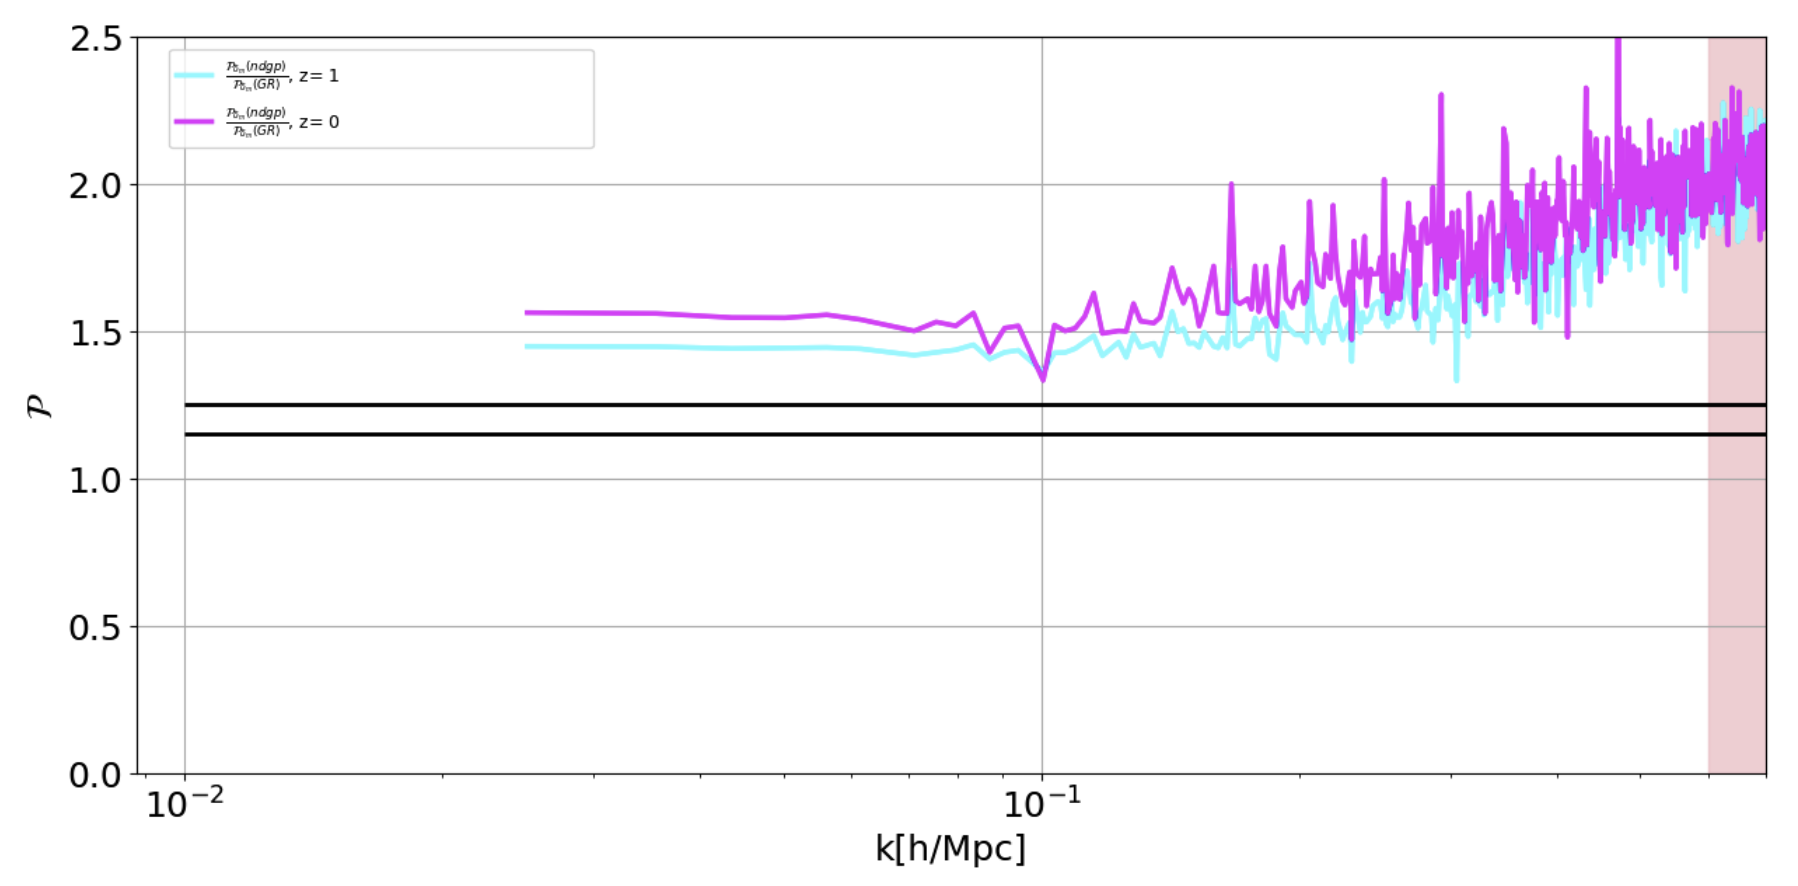
\includegraphics[scale=0.5]{./Images/ndgp_001} 
 \end{figure}
 So we found out the meaning of different $\sigma_8$ comes from just because of different Poisson equation, or modification because of nDGP, which shows itself in the power spectrum and at the end $\sigma_8$ or $A_s$, so now we run for the same cosmological parameters and look at the results,
          \begin{figure}[H]
 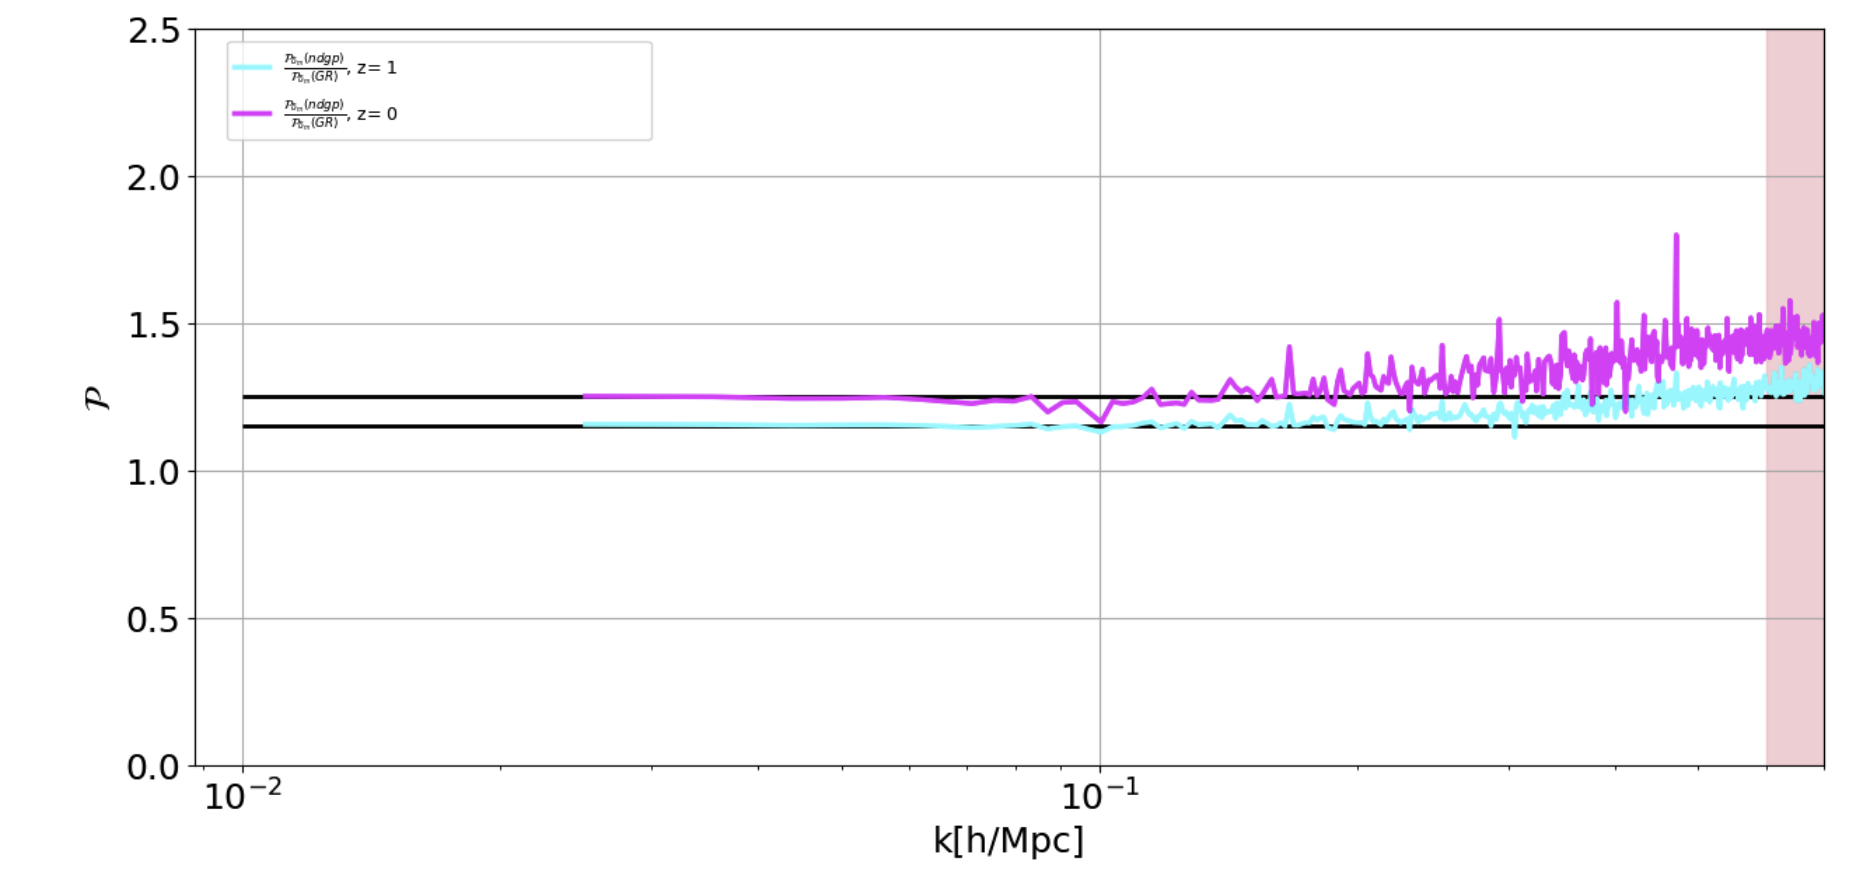
\includegraphics[scale=0.5]{./Images/ndgp_002} 
 \end{figure}
 And because of mode coupling at non-linear regime, we get different grows of perturbations at different scales which is clear in the high-resolution run,
          \begin{figure}[H]
 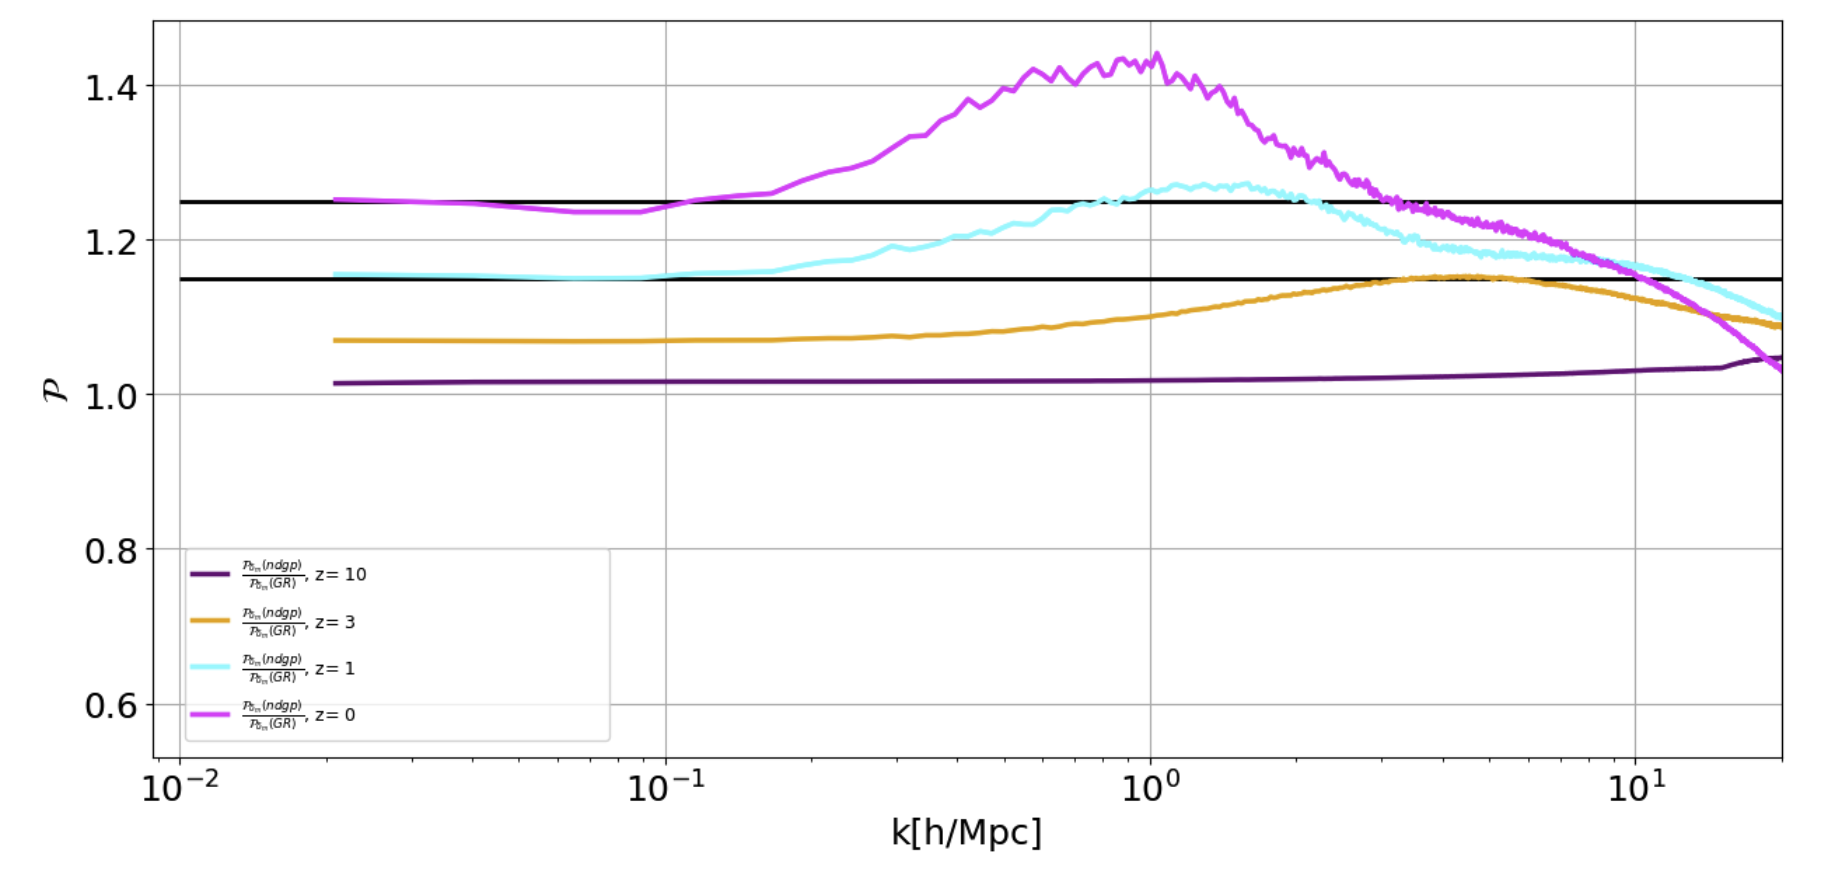
\includegraphics[scale=0.5]{./Images/ndgp_003} 
 \end{figure}
 Compared to the paper result seems correct.
 
         \begin{figure}[H]
 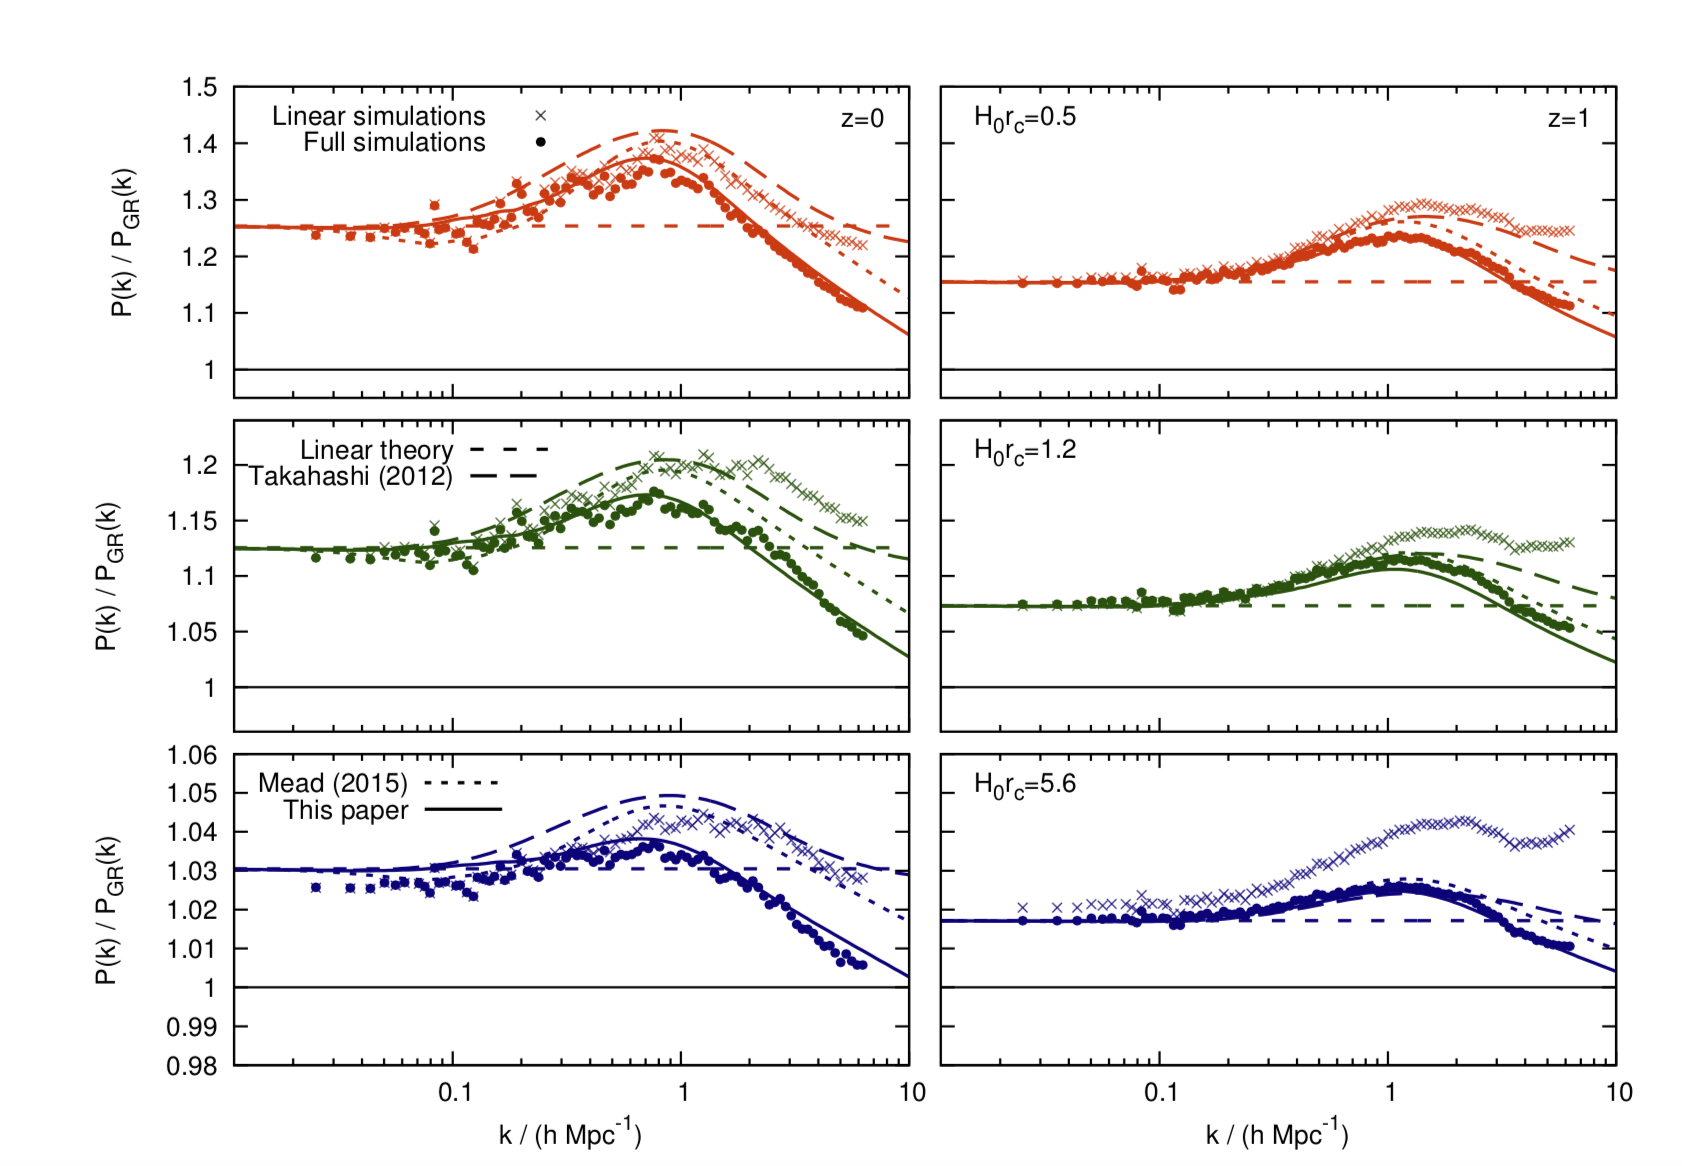
\includegraphics[scale=0.5]{./Images/ndgp_004}  
 \end{figure} 
\section{Screening mechanism}
Now we are going to add screening to the previous results. We follow the same procedure as \url{https://arxiv.org/abs/0911.5178} and \url{https://arxiv.org/pdf/1703.00879.pdf}. Basically because of gravity modification due to scalar field we can write,
\be
\Psi = \Psi_N + \varphi/2
\ee
where,
\be
\nabla^2 \Psi_N = 4 \pi G a^2 \delta \rho
\ee
\be
\nabla^2 \varphi = 8 \pi a^2 \Delta G  \big( \frac{R}{R_*}\big) \delta \rho
\ee
The modified Poisson equation is written,
\be
\nabla^2 \Psi = 4 \pi G a^2 \big( 1+ \frac{\Delta G}{G} \big) \delta \rho
\ee
For the nDGP model $\Delta G$ reads,
\be
\frac{\Delta G}{G } = \frac{2}{3 \beta (a)}   \,\frac{ \sqrt{1+ x^{-3} }-1 }{x^{-3}}
\ee
$R_*$ the Vainstein radius is,
\be
R_* = \Big( \frac{16 G \delta M r_c^2}{9 \beta^2} \Big)
\ee
Moreover,
\be
\delta M= 4 \pi \delta \rho R^3/3
\ee
and  $x= \frac{R}{R_*} $, putting everything together gives,
\be
\epsilon = x^{-3} = \Big(\frac{R_*}{R}\Big)^3 = \frac{8 \HH_0^2 r_c^2}{9 \beta^2} \Omega_m(a) \delta =  \frac{8 \HH_0^2 r_c^2}{9 \beta^2} \Omega_{m,0} a^{-3} \delta
\ee
\be
\frac{\Delta G}{G} = \frac{2}{3 \beta} \frac{ \sqrt{1+\epsilon} -1} {\epsilon}
\ee
\be
\nabla^2 \Psi = 4 \pi G a^2 \big( 1+ \frac{\Delta G}{G} \big) \delta \rho
\ee
In Gevolution we just need to define $\epsilon$ to implement it into the modified Poisson equation,
and $\beta$ is defined as before,
\be
\beta(a) = 1+ \frac{4} {3 a }  \frac{\HH}{\HH_0} \HH_0 r_c    \Big ( 1+ \frac{\HH'}{2 \HH^2} \Big) 
\ee
Note that the $\beta$ in the equation. 10 of \url{https://arxiv.org/pdf/0911.5178.pdf} and equation. 48 of \url{https://arxiv.org/pdf/1602.02154.pdf} are the same.\\
\subsection{Gevolution}
The tricky part to implement in Gevolution is how we read $\delta_m$ in Gevolution. \\
 First note that in  Gevolution $T_0^0 (gev)=-a^3 T_0^0 = -a^3 \big(\bar{\rho} + \delta \rho \big) $ and by definition $ M^2_{pl}= 1/8 \pi G$
Moreover we have we have the following identities,
\be
\Omega_m= \frac{\rho_m(a)}{\rho_{crit} (a)} = \frac{a^2 \bar{\rho}_m(a)}{3 M_{pl}^2 \HH^2}
\ee
\be
\rho_{crit} = \frac{3 M_{pl}^2 \HH^2}{a^2}
\ee
\be
\rho_{crit} ^0= \frac{3 M_{pl}^2 \HH_0^2}{a_0^2}=1
\ee
$\rho^{0}_{crit}=1$ in Gevolution,  i.e. $\HH_0 =H_0 = \frac {8 \pi G}{3} $.\\
%so we can write  $4 \pi G  \rho_m a^2 = 4 \pi G  \frac{\rho_m (a)}{\rho_{cr} (0)} \rho_{cr} (0) a^2 = 4 \pi G  \frac{\Omega_m (0) a^{-3} \rho_{cr}}{\rho_{cr} (0)} \rho_{cr} (0) a^2= (3/2) {H_0}^2   {\Omega_m (0) a^{-3} }  a^2 = ( 3/2) \mathcal{H}_0^2 \Omega_m (0) /a $.\\
On the other hand, $\bar{T}_0^0(Gev) = a^3 \bar{\rho}_m$, so we have,
\be
a^3 \bar{\rho}_m = a^3   \frac{\bar{\rho}_m^0 a^{-3} }{\rho_{crit}^0} {\rho_{crit}^0} = \Omega_m^0
\ee

At the end we can write,
\be
T_0^0 (gev) = \Omega_m^0 \Big( 1+ \delta_m \Big) = a^3 \bar{\rho}_m \big(1+ \delta_m \big)
\ee
\subsection{Relativistic}
So because of the notation in Gevolution, $T_0^0$ is  the perturbation part plus background so,
\be
\delta_m(gev) = \frac{ T_0^0 (gev)  - \bar{T}_0^0 (gev) }{ \bar{T}_0^0 (gev)} = \frac{\text{source}(x) -a^3 \bar{\rho}_m }{ a^3 \bar{\rho}_m } = \frac{\text{source}(x)- \Omega_m^0}{ \Omega_m^0}
\ee

So  $\delta \rho_m$ is exactly $T_0^0 (gev)$ in Gevolution while it is rescaled by $a^3$. To compute $\epsilon$ in the code we need to use $\delta_m =  \frac{ T_0^0 (gev)  - \bar{T}_0^0 (gev) } {  \Omega_m^{0}}$.
So basically having $\delta_m$ we can compute $\epsilon$ easily. \\
$\epsilon$ in Gevolution reads,
\be
\epsilon  =  \frac{8 \HH_0^2 r_c^2}{9 \beta^2} \Omega_{m,0} a^{-3} \delta_m = \frac{8 \HH_0^2 r_c^2}{9 \beta^2} a^{-3}  \Big(T_0^0(gev) -  \bar{T}_0^0 (gev)\Big )
\ee
\subsection{Newtonian}
In the Newtonian Gevolution we have "source(x)" which is actually $\bar{\rho}_m \delta_m =\Omega_m^0 \delta_m = \delta \rho_m$, so $\epsilon$ reads
\be
\epsilon  =  \frac{8 \HH_0^2 r_c^2}{9 \beta^2} \Omega_{m,0} a^{-3} \delta_m =   \frac{8 \HH_0^2 r_c^2}{9 \beta^2} \times  \frac{ \text{source}(x)- \Omega_m^0}{a^3}
\ee
The result is as following, in which we see an offset in the low wavenumbers,
    \begin{figure}[H]
 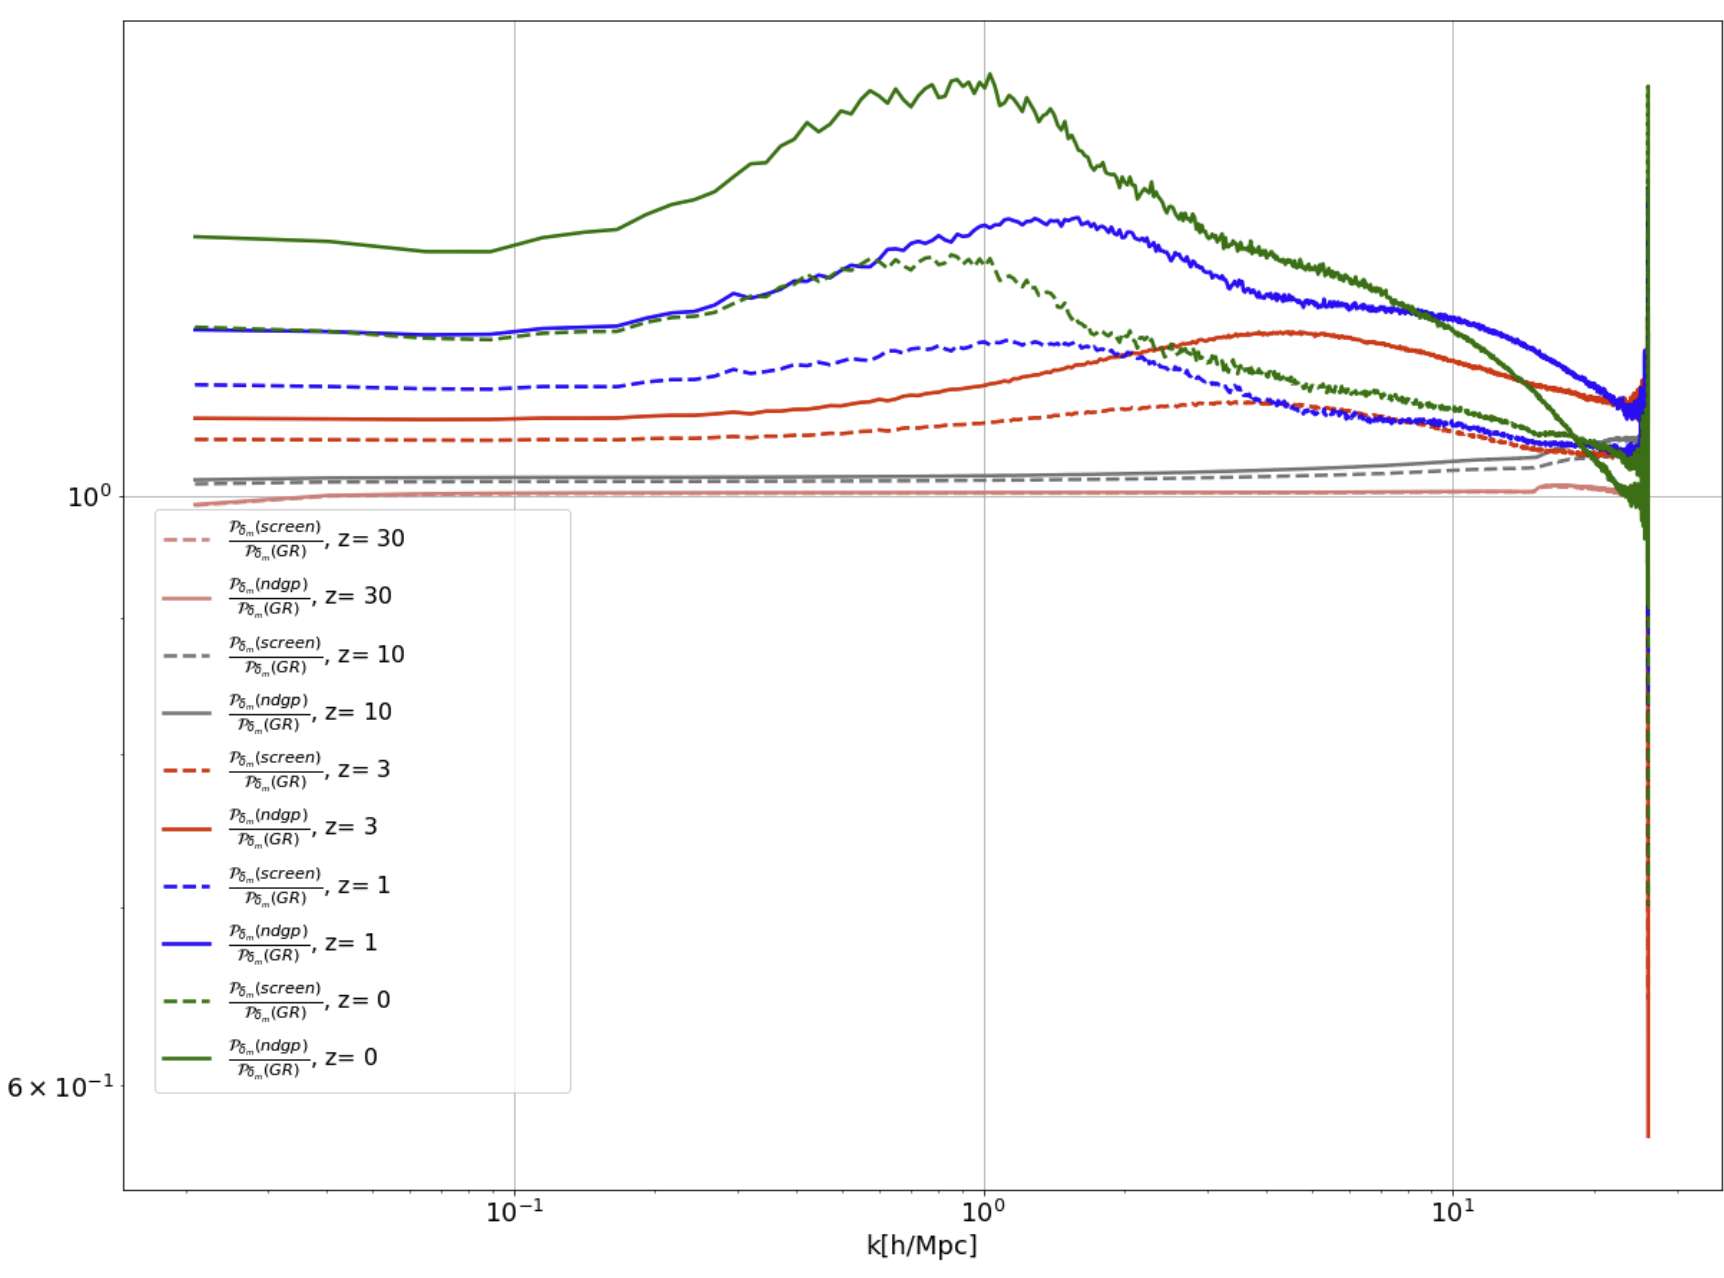
\includegraphics[scale=0.5]{./Images/ndgp_005}  
 \end{figure} 
%Or probably a better way but consistent would be,
%\be
%\epsilon  =  \frac{8 \HH_0^2 r_c^2}{9 \beta^2} \Omega_{m,0} a^{-3} \delta_m =   \frac{8 \HH_0^2 r_c^2}{9 \beta^2} \Omega_{m,0} a^{-3} \frac{\text{source}(x)} {a^3 \bar{\rho}_m}
%\ee
%and reading $ \bar{\rho}_m(a)$ by calculating the average of source field over the lattice.
\section{f(R) gravity}
We follow the same calculation as \url{https://arxiv.org/pdf/0812.0545.pdf} as following,
    \begin{figure}[H]
 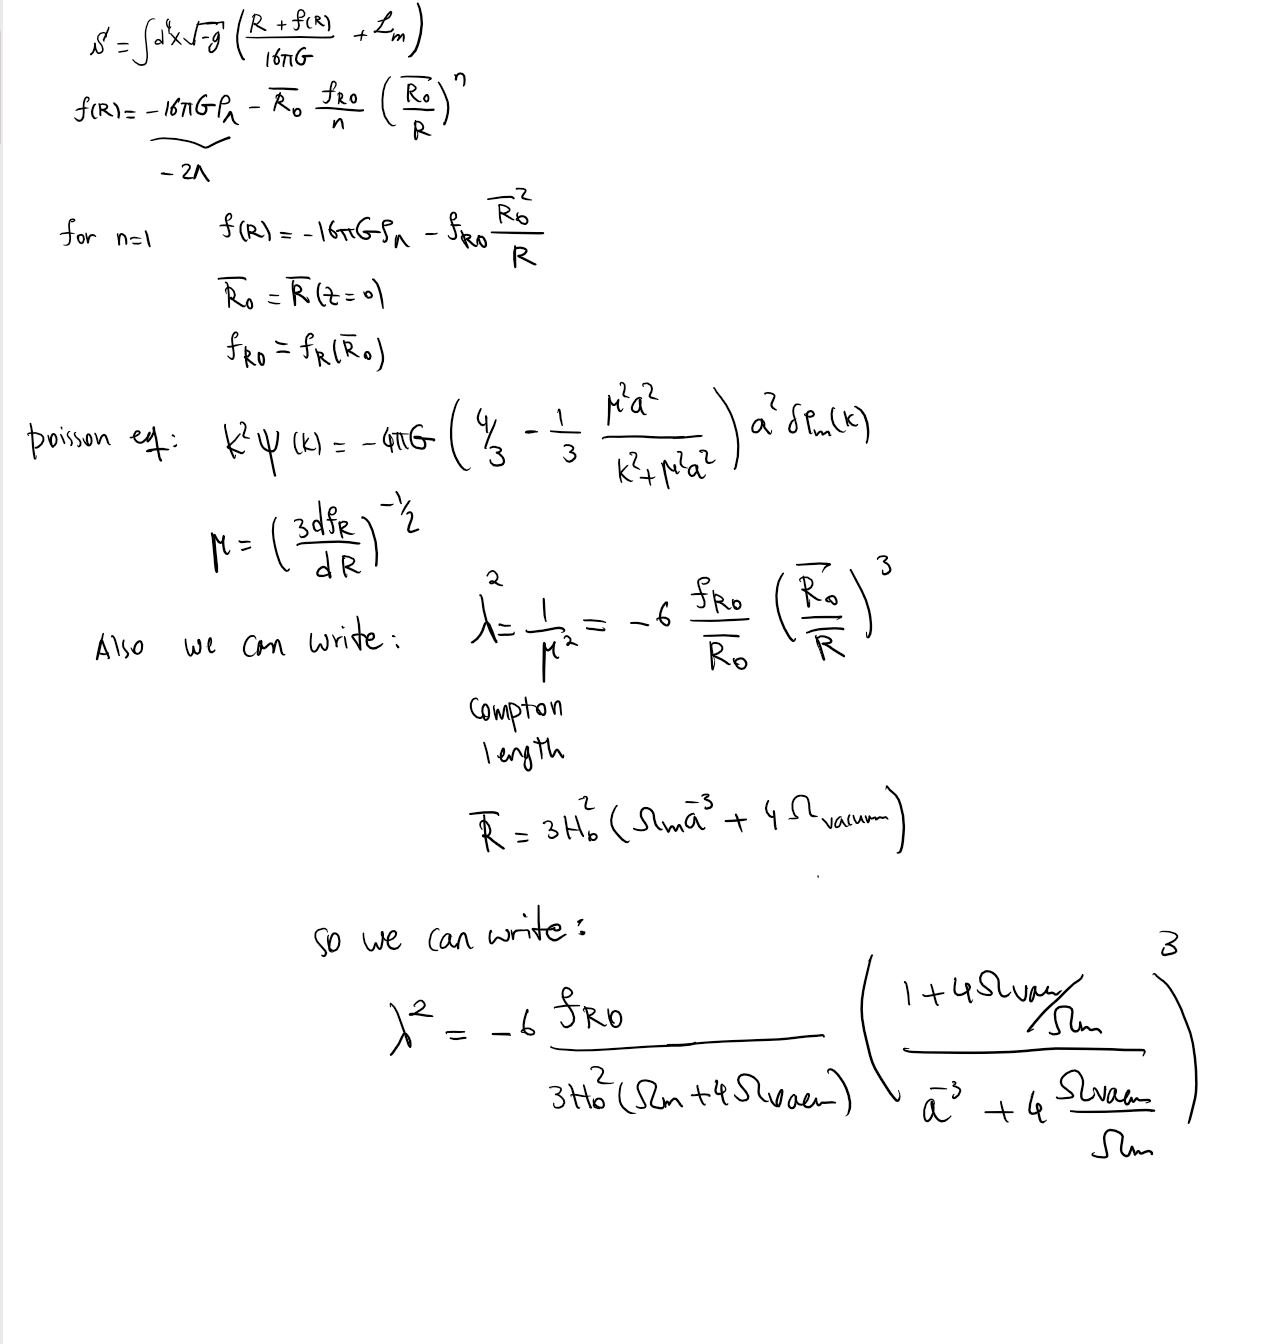
\includegraphics[scale=0.5]{./Images/f(R)}  
 \end{figure} 
 In order to implement it in gevolution.hpp we define a new function as following,
 \lstset {language=python}
\begin{lstlisting}[basicstyle=\tiny,frame=single,
    language=python]
for (int i=0; i<iterations;i++)
{
void solveModifiedPoissonFT_fR(Field<Cplx> & 
sourceFT, Field<Cplx> & potFT, Real coeff, const double fR0, const double a, const double H0 ,const double 
Omega_m ,const double Omega_vacuum ,const Real modif = 0.)
{
	const int linesize = potFT.lattice().size(1);
	int i;
	Real * gridk2;
	Real * sinc;
	rKSite k(potFT.lattice());
  double R_bar = 3. *H0*H0*(Omega_m/a/a/a + 4.*Omega_vacuum);  //Ricci scalar Bg
  double R0_bar = 3. *H0*H0*(Omega_m + 4.*Omega_vacuum);  //Ricci scalar at z=0 Bg
  double f_R_coeff;
  double lambda_squared =  (-6. * fR0/(3.*H0*H0 * (Omega_m+4.*Omega_vacuum))) * 
  pow((Omega_m+4.*Omega_vacuum)/(Omega_m/a/a/a + 4.*Omega_vacuum),3);
   //compton length and =1/mu
  double mu = sqrt(1./lambda_squared);
  double k2;
  // double f_R_modif;
  // f_R_modif

	gridk2 = (Real *) malloc(linesize * sizeof(Real));

	coeff /= -((long) linesize * (long) linesize * (long) linesize);

	for (i = 0; i < linesize; i++)
	{
		gridk2[i] = 2. * (Real) linesize * sin(M_PI * (Real) i / (Real) linesize);
		gridk2[i] *= gridk2[i];
	}
  
	k.first();
	if (k.coord(0) == 0 && k.coord(1) == 0 && k.coord(2) == 0)
	{
		if (modif == 0.)
			potFT(k) = Cplx(0.,0.);
		else
			potFT(k) = sourceFT(k) * coeff / modif;
		k.next();
	}

	for (; k.test(); k.next())
	{
    k2 = gridk2[k.coord(0)] + gridk2[k.coord(1)] + gridk2[k.coord(2)];
    f_R_coeff = 4./3. - (1./3.)*(a*a*mu*mu)/(k2 + mu*mu*a*a);
    potFT(k) = f_R_coeff * sourceFT(k) * coeff /
     (gridk2[k.coord(0)] + gridk2[k.coord(1)] + gridk2[k.coord(2)] + modif);
	}

	free(gridk2);
}
}
\end{lstlisting}
And in the main.cpp we have,
 \lstset {language=python}
\begin{lstlisting}[basicstyle=\tiny,frame=single,
    language=python]
    if (sim.f_R_flag==0)
      {
        solveModifiedPoissonFT(scalarFT, scalarFT, fourpiG / a);  // Newton: phi update (k-space)
      }
      if (sim.f_R_flag==1)
      {
        solveModifiedPoissonFT_fR(scalarFT, scalarFT, fourpiG / a, cosmo.fR0, a, Hconf(1., fourpiG, cosmo) , cosmo.Omega_m , cosmo.Omega_Lambda );
      }
     \end{lstlisting}
     Compared to the paper of Hu and Sawiscki, we get consistent results, but compared to Mattew's results which screening is also included, we have to add Chameleon screening.
         \begin{figure}[H]
 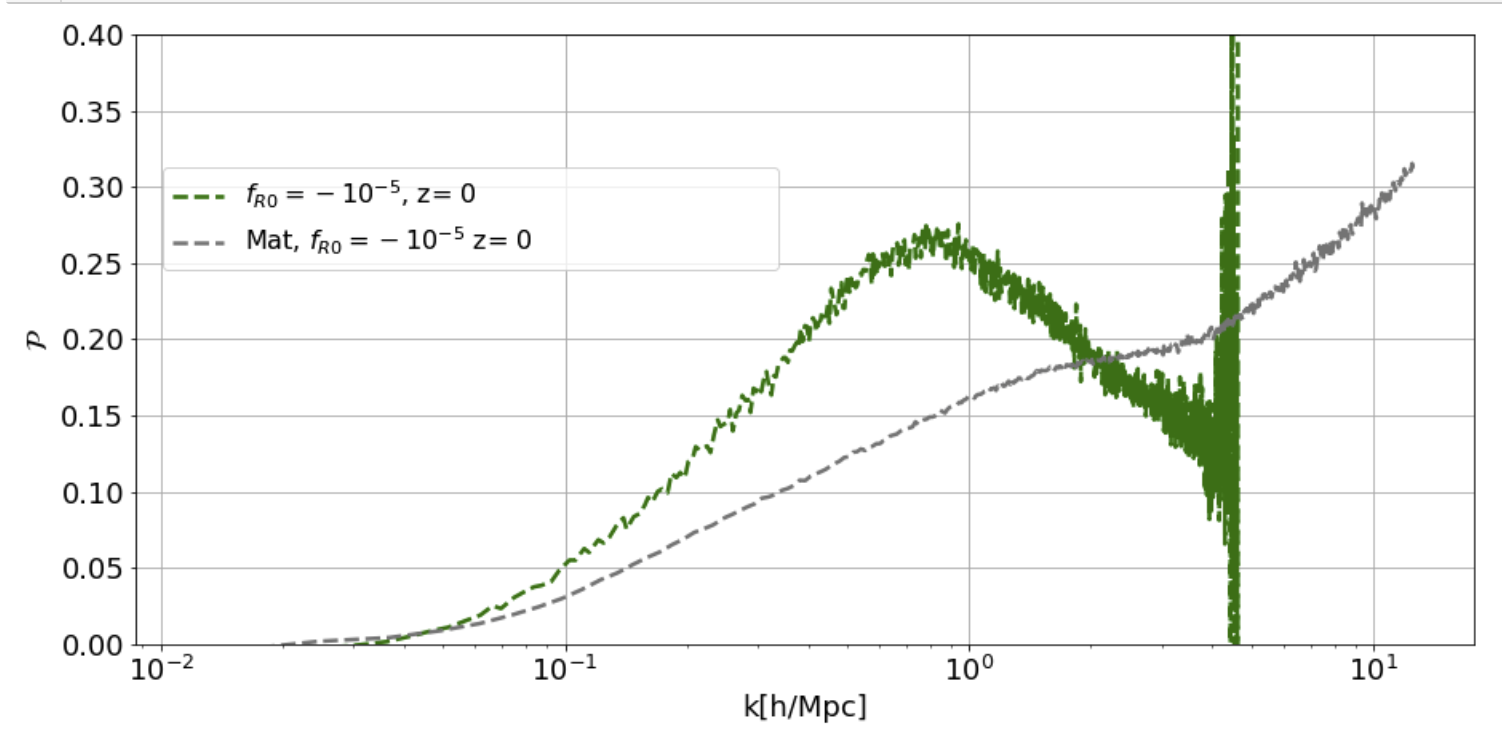
\includegraphics[scale=0.5]{./Images/E-5_z0_fR}  
 \end{figure} 
     \begin{figure}[H]
 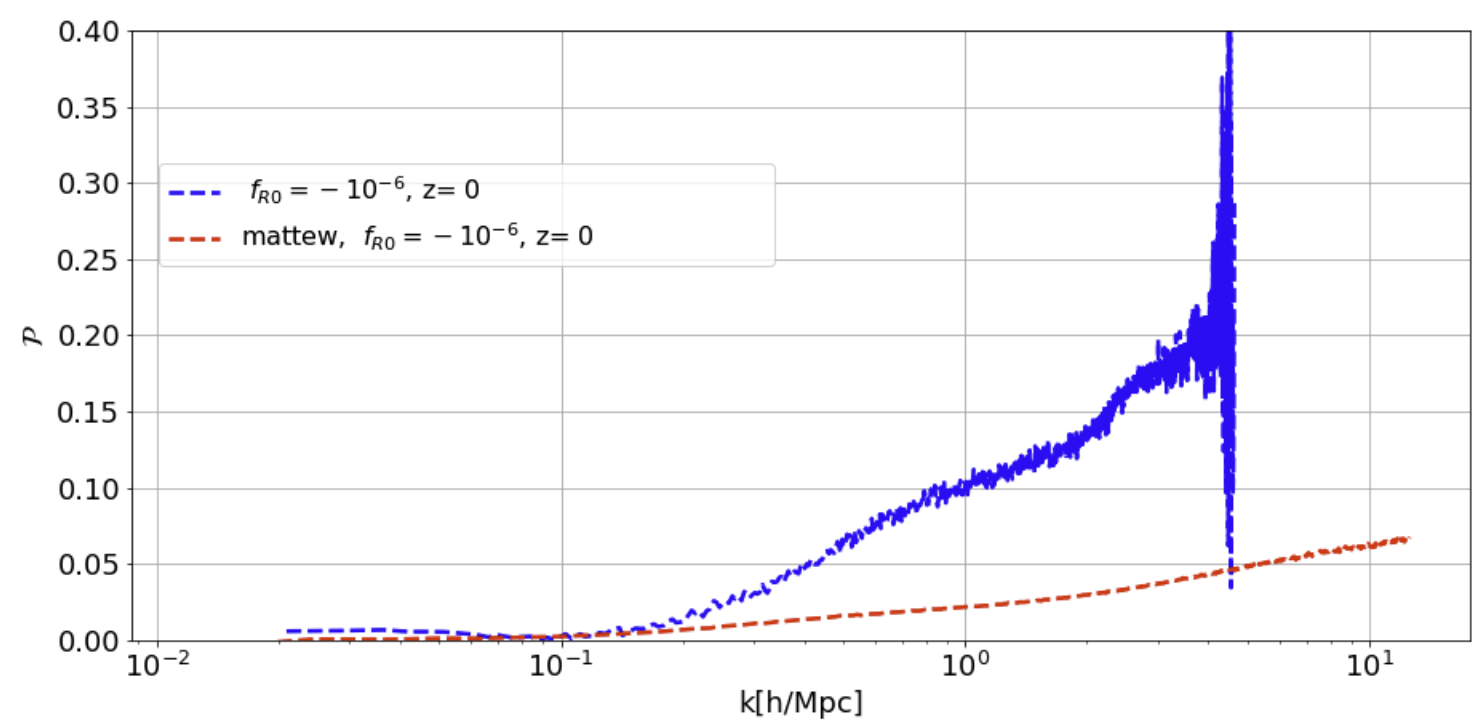
\includegraphics[scale=0.5]{./Images/E-6_z0_fR}  
 \end{figure} 
   

\subsection{Chameleon model}
We use section 5.3 and 5.4 of 1608.00522, having,
\be
\frac{\Delta G_{eff}}{G} = B b \Big (\frac{y_h}{y_0} \Big)^a \Big\{ \big[ 1+ (\frac{y_0}{y_h})^a \big]^{1/b}  -1 \Big\}
\ee
\subsection{General calculation}
Having general $\alpha$ and $w$
\begin{align}
 & p_2 = \frac{\Delta G}{G}, \; \;  p_3 = \frac{4-\alpha}{1-\alpha} = 7,\; \; p_5=-1, \; \; p_6= \frac2 {3 p_3} \\ & \nonumber
 p_7=\frac{3}{\alpha -4 },  \; \; p_4=\Omega_m^{1/3} \Big[ (\Omega_m + 4\Omega_L)^{1/(1-\alpha)}  \frac{b}{3 |f_{R0}|}\Big]^{1/p_3},   \; \;  B = \frac{\Delta G}{G}, \; \; a = \frac{7b}{b-1}
\end{align} 
\be
\frac{\Delta G_{eff}}{G} = \frac{\Delta G}{G} b \Big (\frac{y_h}{y_0} \Big)^{a} \Big\{ \big[ 1+ (\frac{y_0}{y_h})^a \big]^{1/b}  -1 \Big\}
\ee
\begin{align}
y_0  &= p_4 a^{p_5} \Big( 2 G H_0 M_{vir} \Big)^{p_6} \Big(\frac{y_{env}}{y_h} \Big)^{p_7} \nonumber \\ &
=\Omega^{1/3} \Big[ (\Omega_m + 4\Omega_L)^{1/(1-\alpha)}  \frac{b}{3 |f_{R0}|}\Big]^{1/p_3}  a^{-1} \big( 2 G H_0 M_{vir} \big)^{p_6} \Big( \frac{y_{env}}{y_h} \Big)^{p_7}
\end{align}
Having $\epsilon = \Big( \frac{y_{env}}{y_h} \Big)^{p_7}$ , $y_h=\big( \frac{\rho_m^h}{\bar{\rho}_m} \big)^{-1/3}$
\be
\Big(\frac{y_h}{y_0} \Big)^{3} = \frac{\bar{\rho}_m/\rho_m^h}{\Omega_m \Big[ (\Omega_m + 4 \Omega_L) ^{-2} \frac{b}{3 |f_{R_0}|} \Big]^{3/p_3} a^{-3} \big( 2 G H_0 M_{vir} \big)^{3 p_6}  \epsilon ^3}
\ee
\be
\epsilon^{1/p_7} = \Big( \frac{y_{env}}{y_h} \Big) = \frac{\bar{\rho_m}/ \rho_m^{\text{env}}}{\bar{\rho}_m/\rho_m^h} = \frac{\rho_m^h}{\rho_m^{\text{env}}} = \Big( \frac{\zeta_{env}}{\zeta_h} \Big) ^3
\ee
We need to have the following quantities,
\be
M_{vir}, \alpha, b, \rho_m^h, \rho_m^{env}, |f_{R_0}|
\ee
We also assume that the background evolution is not affected, by modified gravity and screening (there is no backreaction). 
 $2 G H_0 M_{vir}$ reads,
 \be
 2 G H_0  M_{vir}  = 2 G H_0   \frac43 \pi \zeta_h^3 \rho^h = \zeta_h^3 H ^2 H_0 \Delta_c
 \ee
 which we have used  $\rho_m^h =\Delta_c \bar{\rho}_c = \frac{3 H^2}{8 \pi G } \Delta_c$. As a result, the following quantities should be given,
 \be
 \zeta^h, \zeta^{env}, b, \alpha, w, \Delta_c
 \ee
 $\bar{\rho}_c$ is the critical density and $\Delta_c$ is a constant given by growth factor and cosmological elements.
 
      \begin{figure}[H]
 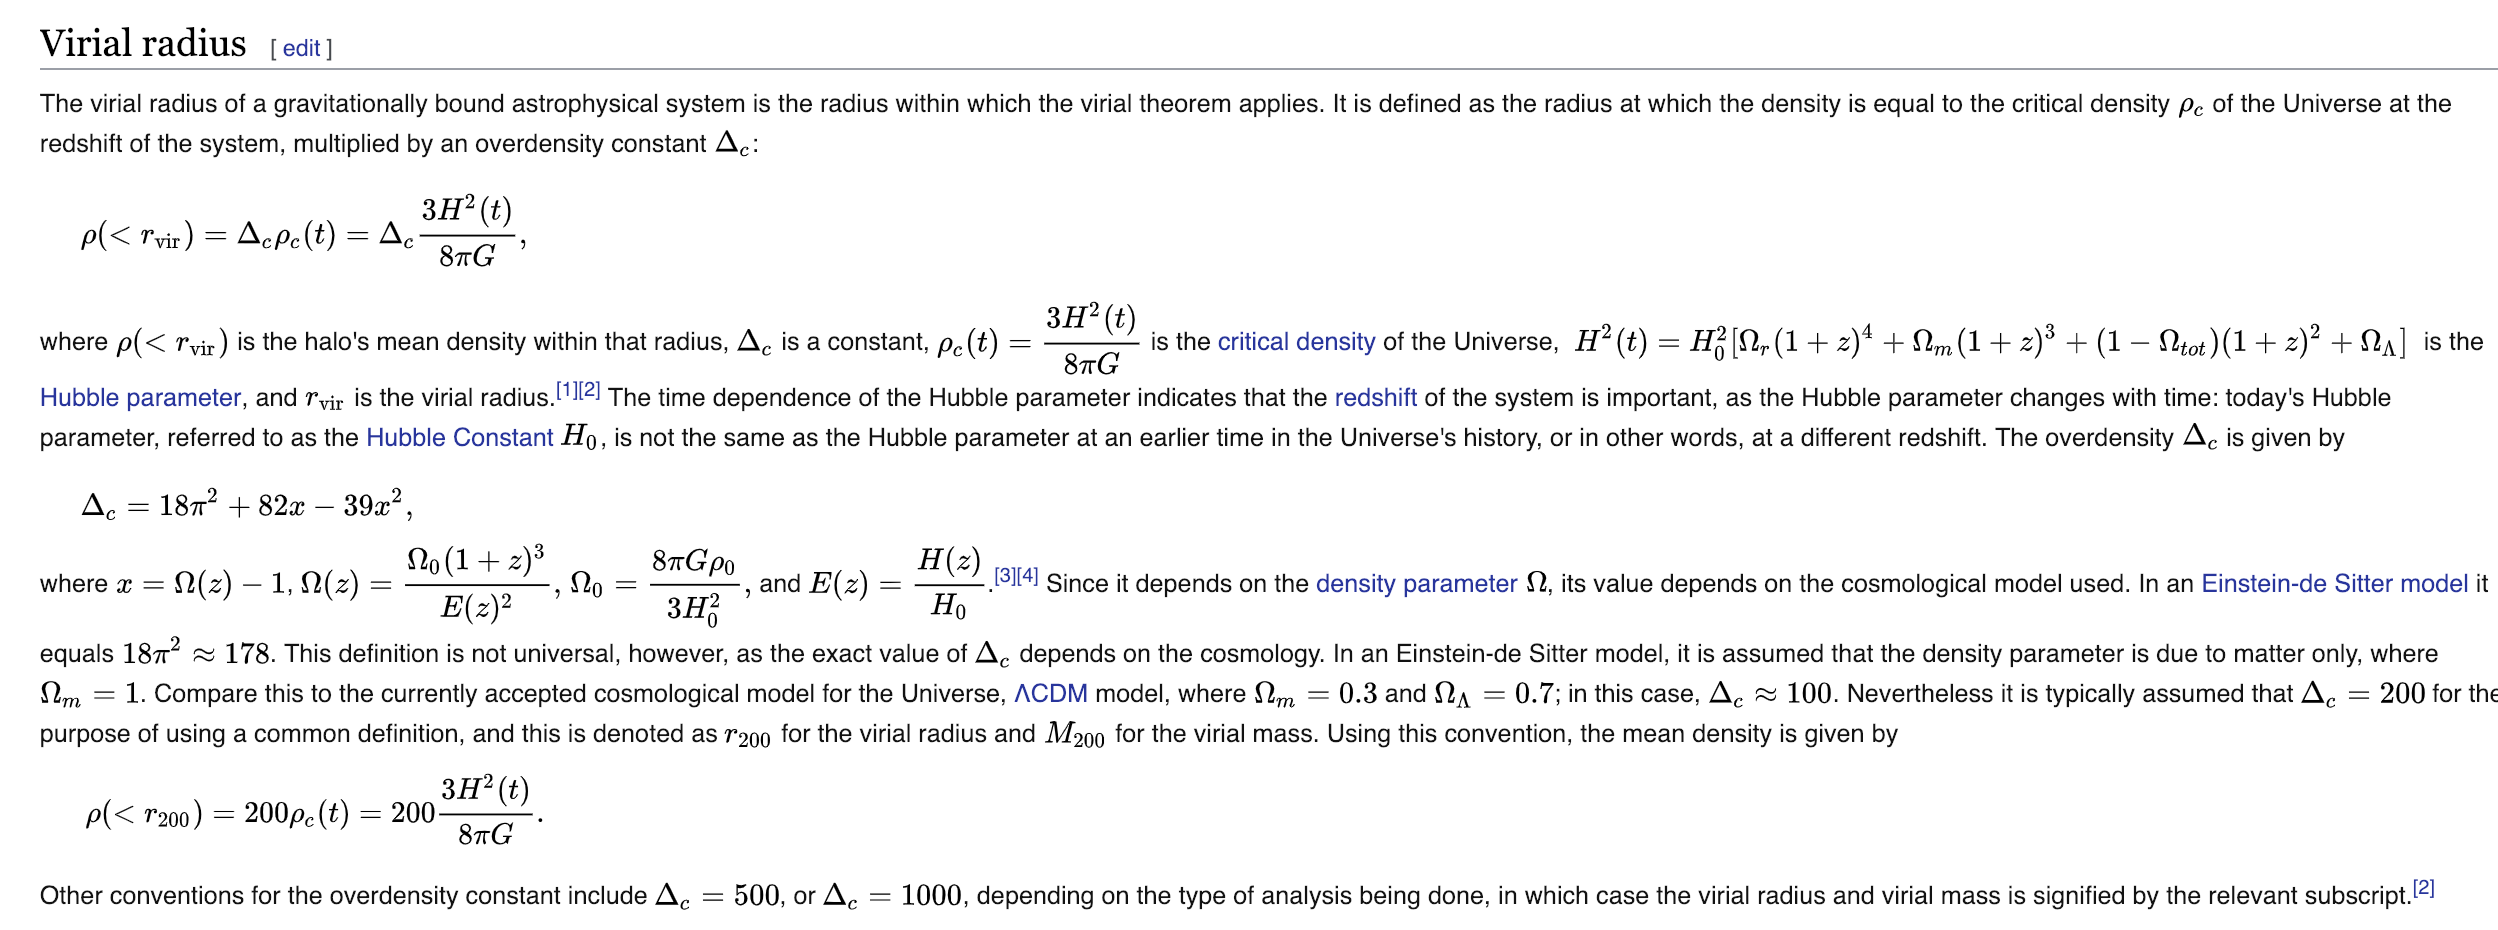
\includegraphics[scale=0.5]{./Images/VirialMass}  
 \end{figure} 
 
 Also 
 \be
 \bar{\rho}_m/\rho_m^h  =  \frac{\bar{\rho}_m/\bar{\rho}_c }{\rho_m^h/\bar{\rho}_c }= \frac{\Omega_m^0 a^{-3}}{\Delta_c}
\ee

\subsection{Choosing $\alpha, w$}
For Chameleon model in the screened regime, for the choice of $p_1=b$ and having,
\begin{align}
& \alpha=\frac12, \; \; w=0 \nonumber \\ & 
 p_2 = \frac{\Delta G}{G}, \; \;  p_3 = \frac{4-\alpha}{1-\alpha} = 7,\; \; p_5=-1, \; \; p_6= \frac2 {21} \\ & \nonumber
 p_7=\frac{-6}{7},  \; \; p_4=\Omega^{1/3} \Big[ (\Omega_m + 4\Omega_L)  \frac{b}{3 |f_{R0}|}\Big]^{1/7},   \; \;  B = \frac{\Delta G}{G}, \; \; a = \frac{7b}{b-1}
\end{align} 
\be
\frac{\Delta G_{eff}}{G} = \frac{\Delta G}{G} b \Big (\frac{y_h}{y_0} \Big)^{\frac{7b}{b-1}} \Big\{ \big[ 1+ (\frac{y_0}{y_h})^{1/2} \big]^{1/b}  -1 \Big\}
\ee
\begin{align}
y_0  &= p_4 a^{p_5} \Big( 2 G H_0 M_{vir} \Big)^{p_6} \Big(\frac{y_{env}}{y_h} \Big)^{p_7} \nonumber \\ &
= \Omega_m^{1/3} \Big[ (\Omega_m + 4 \Omega_L)^{-2} \frac{b}{3|f_{R_0}|} \Big]^{\frac{1}{7}} a^{-1} \big( 2 G H_0 M_{vir} \big)^{\frac{2}{21}} \Big( \frac{y_{env}}{y_h} \Big)^{\frac{-6}{7}}
\end{align}
Having $\epsilon = \Big( \frac{y_{env}}{y_h} \Big)^{-\frac{6}{7}}$ , $y_h=\big( \frac{\rho_m^h}{\bar{\rho}_m} \big)^{-1/3}$
\be
\Big(\frac{y_h}{y_0} \Big)^{3} = \frac{\bar{\rho}_m/\rho_m^h}{\Omega_m \Big[ (\Omega_m + 4 \Omega_L) ^{-2} \frac{b}{3 |f_{R_0}|} \Big]^{3/7} a^{-3} \big( 2 G H_0 M_{vir} \big)^{2/7}  \epsilon ^3}
\ee
\be
\epsilon^{-7/2} = \Big( \frac{y_{env}}{y_h} \Big) = \frac{\bar{\rho_m}/ \rho_m^{\text{env}}}{\bar{\rho}_m/\rho_m^h} = \frac{\rho_m^h}{\rho_m^{\text{env}}}
\ee
Taking $b=6$, $\zeta_h = 1.5 Mpc/h$, $\zeta_{env} = 5 Mpc/h$ we have,
\be
\epsilon = \Big( \frac{\zeta_{env}}{\zeta_h} \Big)^{-6/7}
\ee
Because, $\rho_m^h = M/\zeta_h^3$, $\rho_m^{env} = M/\zeta_{env}^3$.
\subsubsection{Questions:}
- I assumed background quantities ($\Omega_L, \Omega_m$) are at z=0!\\
- We still need to have $\rho^h_m$ or $\delta_m^h$, which I took $\delta_m^h=200$ which is not necessarily true. \\
- What should we do exactly? should we first modify gravity by f(R) in Fourier space then go to real space and screen it? \\
- I think we have to use smoothing in Fourier/ real space to make the densities non-local, inorder to take into account the halos and environments statistically. \\
- Is it ok is to use $\frac{\rho_m^h}{\rho_m^{\text{env}}} = \Big( \frac{\zeta_{env}}{\zeta_h} \Big) ^3$, why? \\
- Should we take $ 2 G H_0  M_{vir} $ where $M_{vir} (z=0)$? I assumed $M_{vir}(z)$! \\
- Do you agree with  $\rho_m^h =\Delta_c \bar{\rho}_c = \frac{3 H^2}{8 \pi G } \Delta_c$ for all halos in average? Can we use it?
- Also we did not use local density in this screening mechanism! I think something is wrong! It would be nice if we could use the local density information by smoothing or something! \\
- Also $\frac{\Delta G_{eff}}{G} = \frac{\Delta G}{G} b \Big (\frac{y_h}{y_0} \Big)^{\frac{7b}{b-1}} \Big\{ \big[ 1+ (\frac{y_0}{y_h})^{1/2} \big]^{1/b}  -1 \Big\}
$ it is not clear what is $ \frac{\Delta G}{G}$, is it ok to do f(R) in Fourier space then go back to real space and apply screening! \\
- Moreover, since we have screening for $\Delta G_{eff}/G$ not for $G_{eff}$ in real space, we really need to have  $\Delta G_{f(R)}/G$ in real space to apply the screening on top of it, while here at most we can have $(1+  \Delta G_{f(R)}/G) * \delta(k)$ then we don't know how to apply screening exactly!  \\
- How to recover f(R) without screening? All the parameters equal to 1, does not work, because we have 1/b-1 in the denominator.



%\begin{lstlisting}[language=C, basicstyle=\tiny]
%scalarProjectionCIC_project(&pcls_cdm, &source);
%void projection_T00_project(Particles<part, part_info, part_dataType> * pcls, Field<Real> * T00, double a = 1., 
%Field<Real> * phi = NULL, double coeff = 1.)
%
%\end{lstlisting}
\section{Implementation}
Since the screening is defined in real space, while we have modified gravity (f(R)) in Fourier space, we first compute the m

The tricky part to implement in Gevolution is how we read $\delta_m$ in Gevolution. \\
 First note that in  Gevolution $T_0^0 (gev)=-a^3 T_0^0 = -a^3 \big(\bar{\rho} + \delta \rho \big) $ and by definition $ M^2_{pl}= 1/8 \pi G$
Moreover we have we have the following identities,
\be
\Omega_m= \frac{\rho_m(a)}{\rho_{crit} (a)} = \frac{a^2 \bar{\rho}_m(a)}{3 M_{pl}^2 \HH^2}
\ee
\be
\rho_{crit} = \frac{3 M_{pl}^2 \HH^2}{a^2}
\ee
\be
\rho_{crit} ^0= \frac{3 M_{pl}^2 \HH_0^2}{a_0^2}=1
\ee
$\rho^{0}_{crit}=1$ in Gevolution,  i.e. $\HH_0 =H_0 = \frac {8 \pi G}{3} $.\\
%so we can write  $4 \pi G  \rho_m a^2 = 4 \pi G  \frac{\rho_m (a)}{\rho_{cr} (0)} \rho_{cr} (0) a^2 = 4 \pi G  \frac{\Omega_m (0) a^{-3} \rho_{cr}}{\rho_{cr} (0)} \rho_{cr} (0) a^2= (3/2) {H_0}^2   {\Omega_m (0) a^{-3} }  a^2 = ( 3/2) \mathcal{H}_0^2 \Omega_m (0) /a $.\\
On the other hand, $\bar{T}_0^0(Gev) = a^3 \bar{\rho}_m$, so we have,
\be
a^3 \bar{\rho}_m = a^3   \frac{\bar{\rho}_m^0 a^{-3} }{\rho_{crit}^0} {\rho_{crit}^0} = \Omega_m^0
\ee

At the end we can write,
\be
T_0^0 (gev) = \Omega_m^0 \Big( 1+ \delta_m \Big) = a^3 \bar{\rho}_m \big(1+ \delta_m \big)
\ee
So because of the notation in Gevolution, $T_0^0$ is  the perturbation part plus background so,
\be
\delta_m(gev) = \frac{ T_0^0 (gev)  - \bar{T}_0^0 (gev) }{ \bar{T}_0^0 (gev)} = \frac{\text{source}(x) -a^3 \bar{\rho}_m }{ a^3 \bar{\rho}_m } = \frac{\text{source}(x)- \Omega_m^0}{ \Omega_m^0}
\ee

So  $\delta \rho_m$ is exactly $T_0^0 (gev)$ in Gevolution while it is rescaled by $a^3$. 
%%%%%%%%%%%%%%%%%%%%%%%%%%%%%
\section{Conclusions}

\setcounter{equation}{0}
%%%%%%%%%%%%%%%%%%%%%

 
\section*{Acknowledgements}

We acknowledge financial support from the Swiss National Science Foundation.


%%%%%%%%%%%%%%%%%%%%%%%%%%%%%%%
%%%%%%%%%%%%%%%%%%%%%%%%%%%%%%%
\appendix
%
\bibliographystyle{JHEP}
%\bibliography{biblio}
\bibliography{EFTDE}


\begin{thebibliography}{999}
\newcommand{\bb}{\bibitem}
%\cite{Hojjati:2011ix}
\bibitem{Hojjati:2011ix}
  A.~Hojjati, L.~Pogosian and G.~B.~Zhao,
  %``Testing gravity with CAMB and CosmoMC,''
  JCAP {\bf 1108} (2011) 005
  doi:10.1088/1475-7516/2011/08/005
  [arXiv:1106.4543 [astro-ph.CO]].
  %%CITATION = doi:10.1088/1475-7516/2011/08/005;%%
  %125 citations counted in INSPIRE as of 20 Sep 2018
 \end{thebibliography}


\end{document}


